% =====================================================================
%  integrales.tex — CDIV — Teórico — Unidad: Integrales
%  Requiere apuntes.sty (estilo/ en la raíz del repo; ver README).
% =====================================================================
\documentclass[11pt,a4paper]{article}
\usepackage{apuntes}

% ---------- Macros propias de esta materia (solo si hacen falta) ----------
% (ninguna por ahora)

% ---------- Metadatos ----------
\materia{CDIV}
\curso{Teórico}
\unidad{Integrales}
\periodo{Clases 10 a 17 --- 2026}
\hypersetup{pdfauthor={Santiago Trujillo}}

\begin{document}
\maketitle
\vspace{-1.6em}
\begin{center}
  {\normalsize Santiago Trujillo\par}
\end{center}
\vspace{0.5em}
\tableofcontents

% =====================================================================
%  CLASES — cada clase nueva se agrega AL FINAL, sin tocar las anteriores
% =====================================================================

% ---------------------------------------------------------------------
\clase{10}{}{Particiones y sumas}
% ---------------------------------------------------------------------

\subsection{Introducción: objetivo y método}

\begin{center}
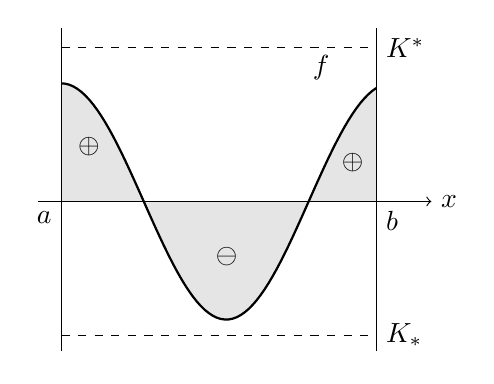
\begin{tikzpicture}
  \fill[gray!20, domain=0:4, samples=80] plot (\x,{1.5*cos(deg(\x*1.5))}) -- (4,0) -- (0,0) -- cycle;
  \draw[->] (-0.3,0) -- (4.7,0) node[right] {$x$};
  \draw (0,-1.9) -- (0,2.2);
  \draw (4,-1.9) -- (4,2.2);
  \draw[thick, domain=0:4, samples=80] plot (\x,{1.5*cos(deg(\x*1.5))});
  \node at (3.3,1.7) {$f$};
  \node[below left] at (0,0) {$a$};
  \node[below right] at (4,0) {$b$};
  \draw[dashed] (0,1.95) -- (4,1.95) node[right] {$K^*$};
  \draw[dashed] (0,-1.7) -- (4,-1.7) node[right] {$K_*$};
  \node at (0.35,0.7) {$\oplus$};
  \node at (2.1,-0.7) {$\ominus$};
  \node at (3.7,0.5) {$\oplus$};
\end{tikzpicture}
\end{center}

\textbf{Objetivo:} medir el área \emph{algebraica} de la región entre el eje $x$ y la gráfica de $f$.

\textbf{Acotación horizontal:} $f\colon[a,b]\to\R$. Se supone que $f$ está acotada:
\[
  K_* \le f(x) \le K^*.
\]

\begin{center}
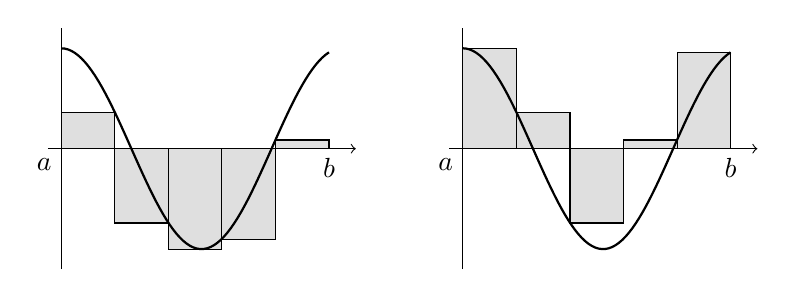
\begin{tikzpicture}[scale=0.85]
  \begin{scope}
    \draw[->] (-0.2,0) -- (4.4,0);
    \draw (0,-1.8) -- (0,1.8);
    \foreach \a/\b/\h in {0/0.8/0.54, 0.8/1.6/-1.11, 1.6/2.4/-1.5, 2.4/3.2/-1.35, 3.2/4/0.13}{
      \fill[gray!25] (\a,0) rectangle (\b,\h);
      \draw (\a,0) rectangle (\b,\h);
    }
    \draw[thick, domain=0:4, samples=80] plot (\x,{1.5*cos(deg(\x*1.5))});
    \node[below left] at (0,0) {$a$};
    \node[below] at (4,0) {$b$};
  \end{scope}
  \begin{scope}[xshift=6cm]
    \draw[->] (-0.2,0) -- (4.4,0);
    \draw (0,-1.8) -- (0,1.8);
    \foreach \a/\b/\h in {0/0.8/1.5, 0.8/1.6/0.54, 1.6/2.4/-1.11, 2.4/3.2/0.13, 3.2/4/1.44}{
      \fill[gray!25] (\a,0) rectangle (\b,\h);
      \draw (\a,0) rectangle (\b,\h);
    }
    \draw[thick, domain=0:4, samples=80] plot (\x,{1.5*cos(deg(\x*1.5))});
    \node[below left] at (0,0) {$a$};
    \node[below] at (4,0) {$b$};
  \end{scope}
\end{tikzpicture}
\end{center}

\begin{center}
\begin{tikzpicture}
  \draw (0,0) rectangle (1.2,1.2);
  \node[below] at (0,0) {$a_i$};
  \node[below] at (1.2,0) {$a_{i+1}$};
  \draw[->] (1.5,0) -- (1.5,1.2) node[midway,right] {$k$};
  \node[right] at (2.2,0.6) {$(a_{i+1}-a_i)\times k$};
  \begin{scope}[xshift=7.5cm]
    \draw (0,0) rectangle (1.2,1.2);
    \node[below] at (0.6,0) {$a$};
    \node[right] at (1.2,0.6) {$h$};
    \node[right, align=left] at (1.9,0.6) {$a\cdot h$\\ $a>0$\\ $h\in\R$};
  \end{scope}
\end{tikzpicture}
\end{center}

$P=\{a_0,\dots,a_n\}$, \qquad $S_*(f,P)$, \qquad $S^*(f,P)$.

\subsection{Particiones de un intervalo}

\begin{definicion}
Una \textbf{partición} de $[a,b]$ (con $a<b$) es un conjunto finito $P\subset[a,b]$ tal que $a\in P$, $b\in P$.
\end{definicion}

\begin{notacion}
$P=\{a_0,a_1,\dots,a_n\}$, con
\[
  a=a_0<a_1<\dots<a_n=b \qquad \text{(siempre se escribe de modo ordenado).}
\]
\end{notacion}

\begin{center}
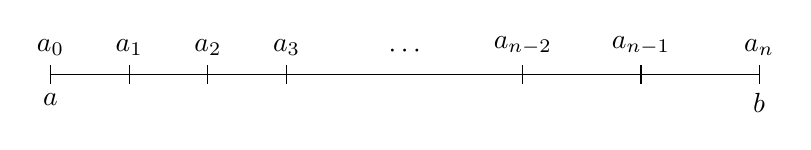
\begin{tikzpicture}
  \draw (0,0) -- (9,0);
  \foreach \x/\l in {0/a_0,1/a_1,2/a_2,3/a_3,6/a_{n-2},7.5/a_{n-1},9/a_n}{
    \draw (\x,0.12) -- (\x,-0.12);
    \node[above] at (\x,0.12) {$\l$};
  }
  \node at (4.5,0.3) {$\cdots$};
  \node[below] at (0,-0.12) {$a$};
  \node[below] at (9,-0.12) {$b$};
\end{tikzpicture}
\end{center}

\[
  [a,b]=\bigcup_{i=0}^{n-1}[a_i,a_{i+1}]
  =[a_0,a_1]\cup[a_1,a_2]\cup\dots\cup[a_{n-1},a_n].
\]

\begin{definicion}[Orden entre las particiones]
$P\subset Q$: $Q$ es \textbf{más fina} que $P$; $P$ es \textbf{más gruesa} que $Q$.
\end{definicion}

\begin{itemize}
  \item Reflexiva: $P\subset P$.
  \item Transitiva: $P\subset Q \wedge Q\subset R \Rightarrow P\subset R$.
  \item Antisimétrica: $P\subset Q \wedge Q\subset P \Rightarrow P=Q$.
\end{itemize}

No es una relación de orden total, pues existen $P,Q\subset[a,b]$ tales que $P\not\subset Q$ y $Q\not\subset P$.

\begin{observacion}\leavevmode
\begin{enumerate}
  \item $P_0=\{a,b\}$ es la partición más gruesa.
  \item Dados $P,Q\subset[a,b]$, la partición $P\cup Q$ es más fina que $P$ y $Q$ a la vez $\Rightarrow$ el \textbf{refinamiento común} ($P$ y $Q$).
\end{enumerate}
\end{observacion}

\begin{definicion}[Norma]
Dado $P=\{a_0,a_1,a_2,\dots,a_n\}$,
\[
  \norm{P} = \max_{i=0,\dots,n-1}\,(a_{i+1}-a_i).
\]
\end{definicion}

\begin{observacion}
$P\subset Q \Rightarrow \norm{Q}\le\norm{P}$.
\end{observacion}

\subsection{Sumas inferiores y superiores}

Sea $f\colon[a,b]\to\R$ acotada:
\[
  K_*\le f(x)\le K^* \qquad (\forall x\in[a,b]).
\]

\begin{notacion}
Dado $[a',b']\subset[a,b]$, se escriben:
\begin{align*}
  \inf\bigl(f,[a',b']\bigr) &:= \inf\{f(x) : x\in[a',b']\},\\
  \sup\bigl(f,[a',b']\bigr) &:= \sup\{f(x) : x\in[a',b']\}.
\end{align*}
\end{notacion}

\begin{minipage}{0.58\textwidth}
Sea $P=\{a_0,a_1,\dots,a_n\}$:
\begin{gather*}
  (a_{i+1}-a_i)\cdot\inf\bigl(f,[a_i,a_{i+1}]\bigr)\\
  (a_{i+1}-a_i)\cdot\sup\bigl(f,[a_i,a_{i+1}]\bigr)
\end{gather*}
\end{minipage}\hfill
\begin{minipage}{0.38\textwidth}
\centering
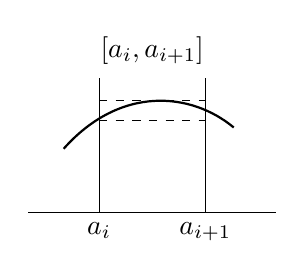
\begin{tikzpicture}[scale=0.9]
  \draw (-0.5,0) -- (3,0);
  \draw (0.5,0) -- (0.5,1.9);
  \draw (2,0) -- (2,1.9);
  \draw[thick] (0,0.9) .. controls (0.8,1.8) and (1.8,1.7) .. (2.4,1.2);
  \draw[dashed] (0.5,1.58) -- (2,1.58);
  \draw[dashed] (0.5,1.3) -- (2,1.3);
  \node[below] at (0.5,0) {$a_i$};
  \node[below] at (2,0) {$a_{i+1}$};
  \node[above] at (1.25,1.95) {$[a_i,a_{i+1}]$};
\end{tikzpicture}
\end{minipage}

\begin{definicion}
Dado $P=\{a_0,a_1,\dots,a_n\}\subset[a,b]$:
\begin{align*}
  S_*(f,P) &= \sum_{i=0}^{n-1}(a_{i+1}-a_i)\cdot\inf\bigl(f,[a_i,a_{i+1}]\bigr),\\
  S^*(f,P) &= \sum_{i=0}^{n-1}(a_{i+1}-a_i)\cdot\sup\bigl(f,[a_i,a_{i+1}]\bigr).
\end{align*}
\end{definicion}

% ---------------------------------------------------------------------
\clase{11}{}{Integral inferior y superior}
% ---------------------------------------------------------------------

\subsection{Partición de un intervalo}

\begin{definicion}
Una partición de $[a,b]$ es un conjunto finito $P\subset[a,b]$ tal que $a\in P$ y $b\in P$.
\end{definicion}

\begin{notacion}
$P=\{a_0,a_1,\dots,a_n\}$ con $a=a_0<a_1<\dots<a_n=b$.
\end{notacion}

\textbf{Orden (parcial):} $P\subset Q \to Q$ más fina que $P$, $P$ más gruesa que $Q$.
\begin{itemize}
  \item Existe una partición más gruesa: $P_0=\{a,b\}$.
  \item Dadas $P,Q\subset[a,b]$ particiones, la partición $P\cup Q$ es más fina que $P$ y $Q$ a la vez (refinamiento común).
\end{itemize}

\subsection{Sumas inferiores y superiores}

Sea $f\colon[a,b]\to\R$ una función acotada:
\[
  \exists\,K_*,K^*\in\R \text{ tales que } K_*\le f(x)\le K^* \quad \forall x\in[a,b].
\]

\begin{center}
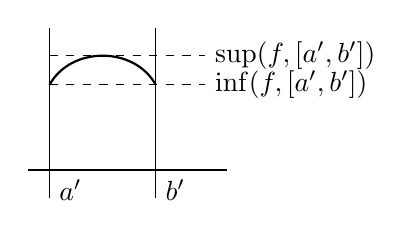
\begin{tikzpicture}[scale=0.9]
  \draw (-0.3,0) -- (2.5,0);
  \draw (0,-0.4) -- (0,2);
  \draw (1.5,-0.4) -- (1.5,2);
  \draw[thick] (0,1.2) .. controls (0.3,1.75) and (1.2,1.75) .. (1.5,1.2);
  \draw[dashed] (0,1.62) -- (2.2,1.62) node[right] {$\sup(f,[a',b'])$};
  \draw[dashed] (0,1.2) -- (2.2,1.2) node[right] {$\inf(f,[a',b'])$};
  \node[below right] at (0,0) {$a'$};
  \node[below right] at (1.5,0) {$b'$};
\end{tikzpicture}
\end{center}

\begin{lema}
Si $[a_2,b_2]\subset[a_1,b_1]\subset[a,b]$, entonces:
\begin{align*}
  \inf\bigl(f,[a_2,b_2]\bigr) &\ge \inf\bigl(f,[a_1,b_1]\bigr),\\
  \sup\bigl(f,[a_2,b_2]\bigr) &\le \sup\bigl(f,[a_1,b_1]\bigr).
\end{align*}
\end{lema}

$A_1=\{f(x):x\in[a_1,b_1]\}$, \quad $A_2=\{f(x):x\in[a_2,b_2]\}$, \quad $A_2\subset A_1$.

\begin{center}
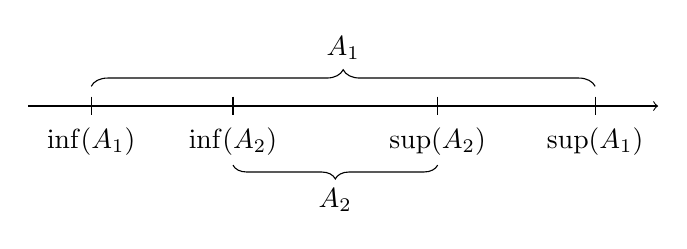
\begin{tikzpicture}
  \draw[->] (0,0) -- (8,0);
  \foreach \x/\l in {0.8/\inf(A_1),2.6/\inf(A_2),5.2/\sup(A_2),7.2/\sup(A_1)}{
    \draw (\x,0.12) -- (\x,-0.12);
    \node[below] at (\x,-0.15) {$\l$};
  }
  \draw[decorate,decoration={brace,amplitude=6pt}] (0.8,0.25) -- (7.2,0.25) node[midway,above=6pt] {$A_1$};
  \draw[decorate,decoration={brace,amplitude=5pt,mirror}] (2.6,-0.75) -- (5.2,-0.75) node[midway,below=5pt] {$A_2$};
\end{tikzpicture}
\end{center}

\begin{definicion}[Sumas inf y sup]
Sea $P=\{a_0,a_1,\dots,a_n\}\subset[a,b]$. Se definen
\begin{center}
$\displaystyle S_*(f,P) := \sum_{i=0}^{n-1}(a_{i+1}-a_i)\cdot\inf\bigl(f,[a_i,a_{i+1}]\bigr)$
\end{center}
\begin{center}
$\displaystyle S^*(f,P) := \sum_{i=0}^{n-1}(a_{i+1}-a_i)\cdot\sup\bigl(f,[a_i,a_{i+1}]\bigr)$
\end{center}
\end{definicion}

\begin{observacion}
$S_*(f,P)\le S^*(f,P)$.
\end{observacion}

\begin{proposicion}
Si $P,Q\subset[a,b]$ son tales que $P\subset Q$:
\[
  \underbrace{S_*(f,P)\le \underbrace{S_*(f,Q)\le S^*(f,Q)}_{Q}\le S^*(f,P)}_{P}.
\]
\end{proposicion}

\begin{demo}
En primer lugar, se considera el caso particular donde $Q=P\cup\{a'\}$ con $a'\notin P$ ($\#(Q\setminus P)=1$). Se puede escribir:
\begin{align*}
  P&=\{a_0,\dots,a_k,a_{k+1},\dots,a_n\},\\
  Q&=\{a_0,\dots,a_k,a',a_{k+1},\dots,a_n\}.
\end{align*}
\begin{align*}
  S_*(f,P) &= \sum_{i=0}^{n-1}(a_{i+1}-a_i)\cdot\inf\bigl(f,[a_i,a_{i+1}]\bigr)\\
  &= S_{i<k} + (a_{k+1}-a_k)\cdot\inf\bigl(f,[a_k,a_{k+1}]\bigr) + S_{i>k}\\
  &= S_{i<k} + \bigl((a'-a_k)+(a_{k+1}-a')\bigr)\cdot\inf\bigl(f,[a_k,a_{k+1}]\bigr) + S_{i>k}\\
  &= S_{i<k} + (a'-a_k)\cdot\inf\bigl(f,[a_k,a_{k+1}]\bigr) + (a_{k+1}-a')\cdot\inf\bigl(f,[a_k,a_{k+1}]\bigr) + S_{i>k}\\
  &\le S_{i<k} + (a'-a_k)\cdot\inf\bigl(f,[a_k,a']\bigr) + (a_{k+1}-a')\cdot\inf\bigl(f,[a',a_{k+1}]\bigr) + S_{i>k}\\
  &= S_*(f,Q).
\end{align*}

\textbf{Caso general:} $Q=P\cup\{a'_1,\dots,a'_p\}$.
\[
  S_*(f,P)\le S_*\bigl(f,P\cup\{a'_1\}\bigr)\le S_*\bigl(f,P\cup\{a'_1,a'_2\}\bigr)\le\dots\le S_*(f,Q).
\]
\end{demo}

\begin{proposicion}
$S_*(f,P)\le S^*(f,Q)$ \quad $\forall\,P,Q\subset[a,b]$.
\end{proposicion}

\begin{demo}
\[
  S_*(f,P)\le S_*(f,P\cup Q)\le S^*(f,P\cup Q)\le S^*(f,Q).
\]
\end{demo}

\subsection{Integral inferior y superior}

Tenemos dos conjuntos de aproximaciones:
\begin{align*}
  A^-(f) &:= \{S_*(f,P) : P\subset[a,b]\},\\
  A^+(f) &:= \{S^*(f,Q) : Q\subset[a,b]\},
\end{align*}
\qquad $A^-(f)\ll A^+(f)$.

\begin{definicion}
\begin{align*}
  I_*(f) &= \sup A^-(f) = \sup_{P\subset[a,b]} S_*(f,P),\\
  I^*(f) &= \inf A^+(f) = \inf_{P\subset[a,b]} S^*(f,P).
\end{align*}
\end{definicion}

\begin{proposicion}
$I_*(f)\le I^*(f)$.
\end{proposicion}

\begin{definicion}
Una función $f\colon[a,b]\to\R$ \emph{acotada} es \textbf{integrable} si $I_*(f)=I^*(f)$.
Cuando es el caso, este número se escribe:
\[
  \int_a^b f \qquad\text{o}\qquad \int_a^b f(x)\dd x.
\]
\end{definicion}

\begin{proposicion}
Sean $f,g\colon[a,b]\to\R$ integrables. Si $f(x)\le g(x)$ $\forall x\in[a,b]$, entonces:
\[
  \int_a^b f\le\int_a^b g.
\]
\end{proposicion}

\begin{demo}
Si $P=\{a_0,a_1,\dots,a_n\}$:
\begin{align*}
  S_*(f,P) &= \sum_{i=0}^{n-1}(a_{i+1}-a_i)\cdot\inf\bigl(f,[a_i,a_{i+1}]\bigr)\\
  &\le \sum_{i=0}^{n-1}(a_{i+1}-a_i)\cdot\inf\bigl(g,[a_i,a_{i+1}]\bigr) = S_*(g,P).
\end{align*}
\begin{gather*}
  S_*(f,P)\le S_*(g,P)\le I_*(g)\\
  \Rightarrow I_*(g) \text{ es cota sup de } \{S_*(f,P) : P\subset[a,b]\}\\
  \Rightarrow I_*(f)\le I_*(g).
\end{gather*}
\end{demo}

% ---------------------------------------------------------------------
\clase{12}{}{Criterios de integrabilidad}
% ---------------------------------------------------------------------

\subsection{Funciones integrables}

\begin{definicion}
Una función $f\colon[a,b]\to\R$ acotada es \textbf{integrable} cuando $I_*(f)=I^*(f)$. Se escribe:
\[
  \int_a^b f=\int_a^b f(x)\dd x := I_*(f)=I^*(f),
  \qquad (b-a)\cdot\inf(f)\le\int_a^b f\le(b-a)\cdot\sup(f).
\]
\end{definicion}

\begin{observacion}
Para toda partición $P\subset[a,b]$:
\[
  S_*(f,P)\le\int_a^b f\le S^*(f,P).
\]
\end{observacion}

Caso particular: $P=\{a,b\}$:
\[
  S_*(f,P)=(b-a)\cdot\inf(f),\qquad S^*(f,P)=(b-a)\cdot\sup(f).
\]

\begin{ejemplo}
Sea una función constante $f\colon[a,b]\to\R$ definida por $f(x)=k$ ($\in\R$).
Sea $P=\{a_0,a_1,\dots,a_n\}\subset[a,b]$. En cada intervalo $[a_i,a_{i+1}]$ leemos que
\[
  \inf\bigl(f,[a_i,a_{i+1}]\bigr)=k,\qquad \sup\bigl(f,[a_i,a_{i+1}]\bigr)=k.
\]
\[
  S_*(f,P)=S^*(f,P)=\sum_{i=0}^{n-1}(a_{i+1}-a_i)\,k
  = k\underbrace{\sum_{i=0}^{n-1}(a_{i+1}-a_i)}_{b-a}=k(b-a).
\]
Tenemos que $I_*(f)=(b-a)\cdot k$, $I^*(f)=(b-a)\cdot k$. Luego
\[
  \int_a^b f=(b-a)\cdot k.
\]
\end{ejemplo}

También existen funciones no integrables:

\begin{ejemplo}
La función de Dirichlet $f\colon[0,1]\to\R$ es definida por:
\[
  f(x)=\begin{cases}1 & \text{si } x\in\Q,\\ 0 & \text{si } x\notin\Q.\end{cases}
\]
Sea $P=\{a_0,\dots,a_n\}\subset[0,1]$. En cada subintervalo $[a_i,a_{i+1}]$:
\[
  \inf\bigl(f,[a_i,a_{i+1}]\bigr)=0,\qquad \sup\bigl(f,[a_i,a_{i+1}]\bigr)=1.
\]
\begin{align*}
  S_*(f,P) &:= \sum_{i=0}^{n-1}(a_{i+1}-a_i)\cdot 0=0,\\
  S^*(f,P) &:= \sum_{i=0}^{n-1}(a_{i+1}-a_i)\cdot 1=b-a=1.
\end{align*}
\begin{center}
\begin{tikzpicture}
  \draw (-0.5,0) -- (5,0);
  \draw (1,0.1) -- (1,-0.1); \draw (3.5,0.1) -- (3.5,-0.1);
  \node[above] at (1,0.1) {$S_*(f,P)$};
  \node[above] at (3.5,0.1) {$S^*(f,P)$};
  \node[below] at (1,-0.1) {$\begin{gathered}0\\ \shortparallel\\ I_*(f)\end{gathered}$};
  \node[below] at (3.5,-0.1) {$\begin{gathered}1\\ \shortparallel\\ I^*(f)\end{gathered}$};
\end{tikzpicture}
\end{center}
$f$ no es integrable.
\end{ejemplo}

\subsection{Criterios de integración}

\begin{observacion}
Para toda partición $P$:
\[
  S_*(f,P)\le I_*(f)\le I^*(f)\le S^*(f,P)
  \;\Rightarrow\; 0\le I^*(f)-I_*(f)\le S^*(f,P)-S_*(f,P).
\]
Más generalmente, si $P\subset Q$:
\[
  0\le I^*(f)-I_*(f)\le S^*(f,Q)-S_*(f,Q)\le S^*(f,P)-S_*(f,P).
\]
\end{observacion}

\begin{proposicion}[Criterio de integración a menos de $\varepsilon$]
Dados una función acotada $f\colon[a,b]\to\R$ y un número $I\in\R$, las siguientes dos condiciones son equivalentes:
\begin{enumerate}
  \item La función $f$ es integrable y tiene integral $\int_a^b f=I$.
  \item Para todo $\varepsilon>0$, existe una partición $P\subset[a,b]$ tal que
  \[
    I-\varepsilon<S_*(f,P)\le S^*(f,P)<I+\varepsilon.
  \]
\end{enumerate}
\end{proposicion}

\begin{demo}
\textbf{(1) $\Rightarrow$ (2).} Supongamos: $I_*(f)=I^*(f)=I$. Sea $\varepsilon>0$.
\begin{itemize}
  \item Como $I=I_*(f)=\sup\{S_*(f,P):P\subset[a,b]\}$, existe una partición $P_1$ tal que $S_*(f,P_1)>I-\varepsilon$.
  \item Como $I=I^*(f)=\inf\{S^*(f,P):P\subset[a,b]\}$, existe otra partición $P_2$ tal que $S^*(f,P_2)<I+\varepsilon$.
\end{itemize}
Sea $P:=P_1\cup P_2$. Tenemos que:
\[
  I-\varepsilon<S_*(f,P_1)\le S_*(f,P)\le S^*(f,P)\le S^*(f,P_2)<I+\varepsilon.
\]

\textbf{(2) $\Rightarrow$ (1).} Supongamos (2). Esto implica que
\[
  I-\varepsilon\le I_*(f)\le I^*(f)<I+\varepsilon \qquad (\forall\varepsilon>0)
\]
\[
  \Rightarrow \abs{I_*(f)-I}<\varepsilon,\qquad \abs{I^*(f)-I}<\varepsilon.
\]
Luego: $I_*(f)=I^*(f)=I$.
\end{demo}

\begin{proposicion}[Criterio de integrabilidad a menos de $\varepsilon$]\mbox{}\\
Dada una función acotada $f\colon[a,b]\to\R$, las siguientes 2 condiciones son equivalentes:
\begin{enumerate}
  \item La función $f$ es integrable en $[a,b]$.
  \item Para todo $\varepsilon>0$, existe $P\subset[a,b]$ tal que
  \[
    0\le S^*(f,P)-S_*(f,P)<\varepsilon.
  \]
\end{enumerate}
\end{proposicion}

\begin{demo}
\textbf{(1) $\Rightarrow$ (2).} Supongamos que $I_*(f)=I^*(f)$. Se escribe $I:=I_*(f)=I^*(f)$.
Sea $\varepsilon>0$. Por el criterio anterior, existe $P\subset[a,b]$ tal que
\[
  I-\tfrac{\varepsilon}{2}<S_*(f,P)\le S^*(f,P)<I+\tfrac{\varepsilon}{2},
\]
\[
  0\le S^*(f,P)-S_*(f,P)<\underbrace{\bigl(I+\tfrac{\varepsilon}{2}\bigr)-\bigl(I-\tfrac{\varepsilon}{2}\bigr)}_{\varepsilon}.
\]

\textbf{(2) $\Rightarrow$ (1).} Supongamos (2). Esto implica que
\[
  0\le I^*(f)-I_*(f)<\varepsilon \qquad (\forall\varepsilon>0).
\]
Luego $I_*(f)=I^*(f)$.
\end{demo}

% ---------------------------------------------------------------------
\clase{13}{}{Monotonía y linealidad}
% ---------------------------------------------------------------------

\subsection{Criterio de integrabilidad}

\begin{proposicion}[Criterio de integrabilidad a menos de $\varepsilon$]\mbox{}\\
Dada una función acotada $f\colon[a,b]\to\R$, las siguientes condiciones son equivalentes:
\begin{enumerate}
  \item $f$ es integrable.
  \item Para todo $\varepsilon>0$, existe una partición $P\subset[a,b]$ tal que $0\le S^*(f,P)-S_*(f,P)<\varepsilon$.
\end{enumerate}
\end{proposicion}

\subsection{Integrabilidad de funciones monótonas}

\begin{teorema}
Si $f\colon[a,b]\to\R$ es monótona creciente o decreciente, entonces es integrable en $[a,b]$.
\end{teorema}

\begin{demo}
Sólo se considera el caso donde $f$ es creciente.
Como $f$ es monótona creciente, está acotada por $f(a)$ y $f(b)$.
Cuando $f(a)=f(b)$, $f$ es constante e integrable.
Ahora, se supone que $f(a)<f(b)$.

Sea $\varepsilon>0$. Sea un entero $n\ge1$ tal que
\[
  \frac{b-a}{n}<\frac{\varepsilon}{f(b)-f(a)}
\]
(tal entero existe por el Principio de Arquímedes).
Sea $P=\{a_0,a_1,\dots,a_n\}$ la partición de $[a,b]$ definida por $a_i=a+i\cdot\dfrac{b-a}{n}$.

\begin{center}
\begin{tikzpicture}[scale=0.9]
  \draw[->] (-0.3,0) -- (5.5,0);
  \draw[->] (0,-0.2) -- (0,3.6);
  \foreach \i in {0,...,5}{ \draw[gray!60] (\i,0) -- (\i,3.4); }
  \foreach \i in {0,...,4}{
    \pgfmathsetmacro{\ya}{0.8+0.09*(\i)^2}
    \pgfmathsetmacro{\yb}{0.8+0.09*(\i+1)^2}
    \fill[blue!20] (\i,\ya) rectangle (\i+1,\yb);
    \draw (\i,\ya) rectangle (\i+1,\yb);
  }
  \draw[thick, domain=0:5, samples=50] plot (\x,{0.8+0.09*\x*\x});
  \node[left] at (0,0.8) {$f(a)$};
  \node[right] at (5,3.05) {$f(b)$};
  \node[below] at (0,0) {$a$};
  \node[below] at (5,0) {$b$};
  \begin{scope}[xshift=7.2cm]
    \foreach \i in {0,...,4}{
      \pgfmathsetmacro{\ya}{0.8+0.09*(\i)^2}
      \pgfmathsetmacro{\yb}{0.8+0.09*(\i+1)^2}
      \fill[blue!20] (0,\ya) rectangle (1,\yb);
      \draw (0,\ya) rectangle (1,\yb);
    }
    \draw[decorate,decoration={brace,amplitude=5pt}] (1.1,3.05) -- (1.1,0.8) node[midway,right=6pt] {$f(b)-f(a)$};
    \node[below] at (0.5,0.7) {$\dfrac{b-a}{n}<\dfrac{\varepsilon}{f(b)-f(a)}$};
  \end{scope}
\end{tikzpicture}
\end{center}

En cada subintervalo $[a_i,a_{i+1}]$:
\begin{align*}
  \inf\bigl(f,[a_i,a_{i+1}]\bigr)&=f(a_i), & S_*(f,P)&=\sum_{i=0}^{n-1}\overbrace{(a_{i+1}-a_i)}^{\frac{b-a}{n}}f(a_i),\\
  \sup\bigl(f,[a_i,a_{i+1}]\bigr)&=f(a_{i+1}), & S^*(f,P)&=\sum_{i=0}^{n-1}(a_{i+1}-a_i)f(a_{i+1}).
\end{align*}
\begin{align*}
  S^*(f,P)-S_*(f,P)&=\sum_{i=0}^{n-1}\Bigl(\frac{b-a}{n}\Bigr)\bigl(f(a_{i+1})-f(a_i)\bigr)\\
  &=\frac{b-a}{n}\sum_{i=0}^{n-1}\bigl(f(a_{i+1})-f(a_i)\bigr)\\
  &=\frac{b-a}{n}\times\bigl(f(b)-f(a)\bigr)<\varepsilon.
\end{align*}
\end{demo}

\begin{ejemplo}
Dado $a>0$, calcular $\displaystyle\int_0^a x^2\dd x$.

\begin{center}
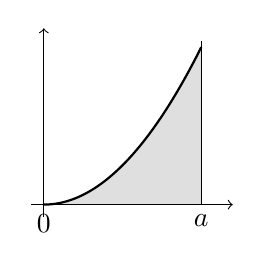
\begin{tikzpicture}[scale=0.8]
  \fill[gray!25, domain=0:2.5, samples=40] (0,0) -- plot (\x,{0.4*\x*\x}) -- (2.5,0) -- cycle;
  \draw[->] (-0.2,0) -- (3,0);
  \draw[->] (0,-0.2) -- (0,2.8);
  \draw (2.5,0) -- (2.5,2.6);
  \draw[thick, domain=0:2.5, samples=40] plot (\x,{0.4*\x*\x});
  \node[below] at (0,0) {$0$};
  \node[below] at (2.5,0) {$a$};
\end{tikzpicture}
\end{center}

\begin{lema}
Si $0\le x\le y$, entonces
\[
  (y-x)\,x^2\le\frac{y^3-x^3}{3}\le(y-x)\,y^2.
\]
\end{lema}

\begin{demo}
$(y^3-x^3)=(y-x)(x^2+xy+y^2)$. Se observa que
\[
  3x^2\le x^2+xy+y^2\le y^2+y^2+y^2=3y^2,
\]
\[
  3(y-x)x^2\le\underbrace{(y-x)(x^2+xy+y^2)}_{y^3-x^3}\le 3(y-x)y^2.
\]
\end{demo}

Sea $P=\{a_0,a_1,\dots,a_n\}\subset[a,b]$.
\[
  S_*(f,P)=\sum_{i=0}^{n-1}(a_{i+1}-a_i)\,a_i^2
  \le\sum_{i=0}^{n-1}\Bigl(\frac{a_{i+1}^3}{3}-\frac{a_i^3}{3}\Bigr)
  =\frac{a_n^3}{3}-\frac{a_0^3}{3}=\frac{a^3}{3}.
\]
Luego: $I_*(f)\le\dfrac{a^3}{3}$.
\[
  S^*(f,P)=\sum_{i=0}^{n-1}(a_{i+1}-a_i)\,a_{i+1}^2
  \ge\sum_{i=0}^{n-1}\Bigl(\frac{a_{i+1}^3}{3}-\frac{a_i^3}{3}\Bigr)=\frac{a^3}{3}.
\]
Luego: $I^*(f)\ge\dfrac{a^3}{3}$. Por lo tanto:
\[
  \int_0^a x^2\dd x=I_*(f)=I^*(f)=\frac{a^3}{3}.
\]
\end{ejemplo}

\subsection{Monotonía de la integral}

\begin{proposicion}[Monotonía de la integral]
Sean $f,g\colon[a,b]\to\R$ dos funciones integrables. Si $\underbrace{f(x)\le g(x)\ (\forall x\in[a,b])}_{f\le g}$, entonces
\[
  \int_a^b f\le\int_a^b g.
\]
\end{proposicion}

\begin{corolario}
$f\ge0\Rightarrow\displaystyle\int_a^b f\ge0$; \qquad $f\le0\Rightarrow\displaystyle\int_a^b f\le0$.
\end{corolario}

\begin{observacion}\leavevmode
\begin{center}
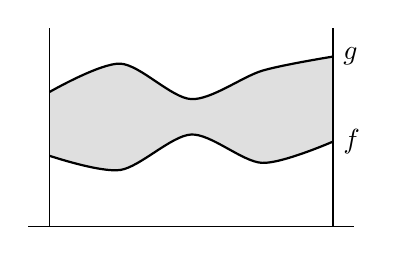
\begin{tikzpicture}[scale=0.9]
  \fill[gray!25] plot[smooth] coordinates {(0,1.9) (1,2.3) (2,1.8) (3,2.2) (4,2.4)}
     -- plot[smooth] coordinates {(4,1.2) (3,0.9) (2,1.3) (1,0.8) (0,1)} -- cycle;
  \draw[thick] plot[smooth] coordinates {(0,1.9) (1,2.3) (2,1.8) (3,2.2) (4,2.4)} node[right] {$g$};
  \draw[thick] plot[smooth] coordinates {(0,1) (1,0.8) (2,1.3) (3,0.9) (4,1.2)} node[right] {$f$};
  \draw (-0.3,0) -- (4.3,0);
  \draw (0,0) -- (0,2.8); \draw (4,0) -- (4,2.8);
\end{tikzpicture}
\end{center}
\[
  \text{área}=\int_a^b g-\int_a^b f \quad\Bigl(=\int_a^b(g-f)\Bigr).
\]
\end{observacion}

$f,g\colon[-1,1]\to\R$, \quad $f(x)=\sqrt{1-x^2}$, \quad $g(x)=-f(x)$.
\begin{center}
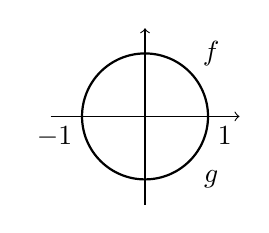
\begin{tikzpicture}[scale=0.8]
  \draw[->] (-1.5,0) -- (1.5,0);
  \draw[->] (0,-1.4) -- (0,1.4);
  \draw[thick] (0,0) circle (1);
  \node[below left] at (-1,0) {$-1$};
  \node[below right] at (1,0) {$1$};
  \node at (1.05,1.0) {$f$};
  \node at (1.05,-1.0) {$g$};
\end{tikzpicture}
\end{center}

\subsection{Linealidad de la integral}

\begin{teorema}
Sean $f,g\colon[a,b]\to\R$ integrables.
\begin{enumerate}
  \item $f+g$ es integrable, y $\displaystyle\int_a^b(f+g)=\int_a^b f+\int_a^b g$.
  \item Para todo $\alpha\in\R$, $\alpha f$ es integrable y $\displaystyle\int_a^b\alpha f=\alpha\int_a^b f$.
\end{enumerate}
\end{teorema}

\begin{observacion}
El conjunto $\mathcal{F}([a,b],\R)$ es un espacio vectorial.
\begin{center}
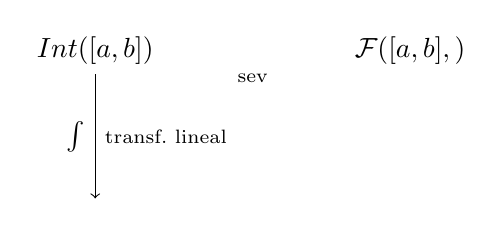
\begin{tikzpicture}
  \node (I) at (0,0) {$\operatorname{Int}([a,b])$};
  \node (F) at (4,0) {$\mathcal{F}([a,b],\R)$};
  \node at (2,0) {$\subsetneq$};
  \node[font=\scriptsize] at (2,-0.35) {sev};
  \node (R) at (0,-2) {$\R$};
  \draw[->] (I) -- (R) node[midway,left] {$\int$} node[midway,right,font=\scriptsize] {transf.\ lineal};
\end{tikzpicture}
\end{center}

\begin{center}
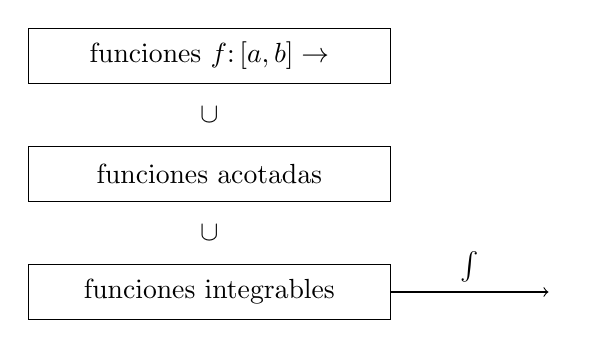
\begin{tikzpicture}[box/.style={draw, minimum width=4.6cm, minimum height=0.7cm}]
  \node[box] (a) at (0,0) {funciones $f\colon[a,b]\to\R$};
  \node at (0,-0.75) {$\cup$};
  \node[box] (b) at (0,-1.5) {funciones acotadas};
  \node at (0,-2.25) {$\cup$};
  \node[box] (c) at (0,-3) {funciones integrables};
  \draw[->] (c.east) -- ++(2,0) node[midway,above] {$\int$} node[right] {$\R$};
\end{tikzpicture}
\end{center}
\end{observacion}

% ---------------------------------------------------------------------
\clase{14}{}{Linealidad y valor absoluto}
% ---------------------------------------------------------------------

\subsection{Linealidad}

\begin{teorema}
Sean $f,g\colon[a,b]\to\R$ integrables. Entonces:
\begin{enumerate}
  \item $f+g$ es integrable y $\displaystyle\int_a^b(f+g)=\int_a^b f+\int_a^b g$.
  \item Para todo $\alpha\in\R$, $\alpha f$ es integrable y $\displaystyle\int_a^b(\alpha f)=\alpha\int_a^b f$.
\end{enumerate}
\end{teorema}

\subsubsection*{(1) Aditividad}

\begin{lema}
Sean $f,g\colon[a,b]\to\R$ acotadas. Entonces para todo subintervalo $[a',b']\subset[a,b]$:
\begin{align*}
  \inf\bigl(f+g,[a',b']\bigr)&\ge\inf\bigl(f,[a',b']\bigr)+\inf\bigl(g,[a',b']\bigr),\\
  \sup\bigl(f+g,[a',b']\bigr)&\le\sup\bigl(f,[a',b']\bigr)+\sup\bigl(g,[a',b']\bigr).
\end{align*}
\end{lema}

\begin{demo}[Demostración de (1)]
Usando el lema anterior, se verifica que
\[
  \left.\begin{aligned}
    S_*(f+g,P)&\ge S_*(f,P)+S_*(g,P)\\
    S^*(f+g,P)&\le S^*(f,P)+S^*(g,P)
  \end{aligned}\right\}\quad\text{para toda partición } P\subset[a,b].
\]
Queremos demostrar que
\[
  I_*(f+g)\ge I_*(f)+I_*(g),\qquad I^*(f+g)\le I^*(f)+I^*(g).
\]
Sea $\varepsilon>0$, se consideran
\begin{itemize}
  \item una partición $P_1\subset[a,b]$ tal que $S_*(f,P_1)>I_*(f)-\varepsilon/2$;
  \item una partición $P_2\subset[a,b]$ tal que $S_*(g,P_2)>I_*(g)-\varepsilon/2$.
\end{itemize}
Sea $P:=P_1\cup P_2$.
\begin{center}
$I_*(f)+I_*(g)-\varepsilon < S_*(f,P_1)+S_*(g,P_2)\le$ $S_*(f,P)+S_*(g,P)$\\[4pt]
$\le S_*(f+g,P)\le I_*(f+g)$.
\end{center}
Demostramos que $I_*(f)+I_*(g)\le I_*(f+g)+\varepsilon$ $\forall\varepsilon>0$.

Ahora, si $f$ y $g$ son integrables, tenemos que $I_*(f)=I^*(f)$ y $I_*(g)=I^*(g)$. Luego:
\begin{align*}
  \int_a^b f+\int_a^b g&=I_*(f)+I_*(g)\le I_*(f+g)\le I^*(f+g)\\
  &\le I^*(f)+I^*(g)=\int_a^b f+\int_a^b g.
\end{align*}
\end{demo}

\subsubsection*{(2) Homogeneidad}

Se distinguen 3 casos:
\begin{itemize}
  \item Caso donde $\alpha=0$: $\displaystyle\int_a^b 0\cdot f=0=0\cdot\int_a^b f$.
  \item Caso donde $\alpha>0$: se verifica fácilmente que
  \[
    \left.\begin{aligned}
      S_*(\alpha f,P)&=\alpha\cdot S_*(f,P)\\
      S^*(\alpha f,P)&=\alpha\cdot S^*(f,P)
    \end{aligned}\right\}\quad\text{para toda partición } P\subset[a,b],
  \]
  y se deduce: $I_*(\alpha f)=\alpha\cdot I_*(f)$, $I^*(\alpha f)=\alpha\cdot I^*(f)$.
  Como $f$ es integrable:
  \[
    I_*(\alpha f)=\alpha\cdot I_*(f)=\alpha\int_a^b f=\alpha\cdot I^*(f)=I^*(\alpha f).
  \]
  \item Caso donde $\alpha<0$:
  \begin{align*}
    S_*(\alpha f,P)&=\alpha\cdot S^*(f,P) &&\rightsquigarrow & I_*(\alpha f)&=\alpha\, I^*(f),\\
    S^*(\alpha f,P)&=\alpha\cdot S_*(f,P) &&\rightsquigarrow & I^*(\alpha f)&=\alpha\, I_*(f).
  \end{align*}
  \[
    I_*(\alpha f)=\alpha\cdot I^*(f)=\alpha\int_a^b f=\alpha\cdot I_*(f)=I^*(\alpha f).
  \]
\end{itemize}

\begin{corolario}[Combinaciones lineales]
Si $f_1,\dots,f_n\colon[a,b]\to\R$ son integrables, entonces para todos $\alpha_1,\dots,\alpha_n\in\R$, la función $\alpha_1f_1+\dots+\alpha_nf_n$ es integrable, y:
\[
  \int_a^b(\alpha_1f_1+\dots+\alpha_nf_n)=\alpha_1\int_a^b f_1+\dots+\alpha_n\int_a^b f_n.
\]
\end{corolario}

Caso particular: si $f\le g$,

\begin{minipage}{0.6\textwidth}
\[
  \text{área}(R)=\int_a^b g-\int_a^b f=\int_a^b(g-f).
\]
\end{minipage}\hfill
\begin{minipage}{0.35\textwidth}
\centering
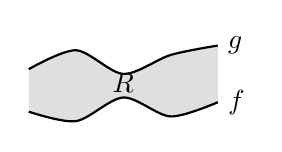
\begin{tikzpicture}[scale=0.6]
  \fill[gray!25] plot[smooth] coordinates {(0,1.9) (1,2.3) (2,1.8) (3,2.2) (4,2.4)}
     -- plot[smooth] coordinates {(4,1.2) (3,0.9) (2,1.3) (1,0.8) (0,1)} -- cycle;
  \draw[thick] plot[smooth] coordinates {(0,1.9) (1,2.3) (2,1.8) (3,2.2) (4,2.4)} node[right] {$g$};
  \draw[thick] plot[smooth] coordinates {(0,1) (1,0.8) (2,1.3) (3,0.9) (4,1.2)} node[right] {$f$};
  \node at (2,1.6) {$R$};
\end{tikzpicture}
\end{minipage}

\subsection{Integral y valor absoluto}

\begin{center}
\begin{tikzpicture}[scale=0.9]
  \begin{scope}
    \fill[gray!25, domain=0:4, samples=60] plot (\x,{0.9*sin(deg(\x*1.3+0.3))}) -- (4,0) -- (0,0) -- cycle;
    \draw (-0.2,0) -- (4.2,0); \draw (0,-1.1) -- (0,1.1); \draw (4,-1.1) -- (4,1.1);
    \draw[thick, domain=0:4, samples=60] plot (\x,{0.9*sin(deg(\x*1.3+0.3))});
    \node at (0.5,0.35) {\scriptsize$+$};
    \node at (2.3,-0.4) {\scriptsize$-$};
    \node at (3.7,0.35) {\scriptsize$+$};
    \node[right] at (4.3,0.2) {$\displaystyle\int_a^b f=\text{área algebraica}$};
  \end{scope}
  \begin{scope}[yshift=-2.6cm]
    \fill[gray!25, domain=0:4, samples=60] plot (\x,{abs(0.9*sin(deg(\x*1.3+0.3)))}) -- (4,0) -- (0,0) -- cycle;
    \draw (-0.2,0) -- (4.2,0); \draw (0,0) -- (0,1.1); \draw (4,0) -- (4,1.1);
    \draw[thick, domain=0:4, samples=60] plot (\x,{abs(0.9*sin(deg(\x*1.3+0.3)))});
    \node at (-0.4,0.8) {$\abs{f}$};
    \node[right, align=left] at (4.3,0.4) {$\abs{f}\colon[a,b]\to\R$\\ $\abs{f}(x)=\abs{f(x)}$};
  \end{scope}
\end{tikzpicture}
\end{center}

\begin{definicion}
Dada $f\colon[a,b]\to\R$:
\begin{itemize}
  \item Se llama \textbf{parte positiva} de $f$ a la función $f^+\colon[a,b]\to\R$ definida por
  \[
    f^+(x)=\max\bigl(0,f(x)\bigr).
  \]
  \item \textbf{Parte negativa:} $f^-(x):=(-f)^+$.
\end{itemize}
\end{definicion}

\begin{observacion}\leavevmode
\begin{itemize}
  \item $f^+,f^-\ge0$.
  \item $f=f^+-f^-$.
  \item $\abs{f}=f^++f^-$.
\end{itemize}
\end{observacion}

\begin{lema}
$f\colon[a,b]\to\R$ integrable $\Rightarrow$ $f^+,f^-\colon[a,b]\to\R$ integrables.
\end{lema}

\begin{idea}
\[
  0\le S^*(f^+,P)-S_*(f^+,P)\le S^*(f,P)-S_*(f,P)\qquad\text{para toda partición } P\subset[a,b].
\]
Luego: $f^-=(-f)^+$.
\end{idea}

\begin{proposicion}
Si $f\colon[a,b]\to\R$ es integrable, entonces $\abs{f}$ también es integrable y
\[
  \abs[\Big]{\int_a^b f}\le\int_a^b\abs{f}.
\]
\end{proposicion}

\begin{demo}
$f$ es integrable, luego $f^+,f^-$ son integrables.
\begin{align*}
  \abs[\Big]{\int_a^b f} &= \abs[\Big]{\int_a^b(f^+-f^-)} = \abs[\Big]{\int_a^b f^+-\int_a^b f^-}
  \le\abs[\Big]{\int_a^b f^+}+\abs[\Big]{-\int_a^b f^-}\\
  &= \int_a^b f^++\int_a^b f^- = \int_a^b(f^++f^-) = \int_a^b\abs{f}.
\end{align*}
\end{demo}

\subsection{Aditividad respecto al intervalo}

\begin{proposicion}
Si $f\colon[a,b]\to\R$ es integrable en $[a,b]$, entonces también es integrable en cualquier subintervalo $[a',b']\subset[a,b]$ ($a\le a'<b'\le b$).
\end{proposicion}

\begin{definicion}
Sea $f\colon I\to\R$ definida en un intervalo $I\subset\R$ cualquiera. Se dice que $f$ es \textbf{localmente integrable} si es integrable en todo subintervalo $[a,b]\subset I$ (con $a<b$).
\end{definicion}

\begin{proposicion}
Sean $f\colon I\to\R$ definida en un intervalo $I\subset\R$ y $a,b,c\in I$ tales que $a<b<c$. Si $f$ es integrable en ambos intervalos $[a,b]$ y $[b,c]$, entonces $f$ es integrable en $[a,c]$. Además
\[
  \int_a^c f=\int_a^b f+\int_b^c f.
\]
\end{proposicion}

% ---------------------------------------------------------------------
\clase{15}{}{Aditividad y funciones escalonadas}
% ---------------------------------------------------------------------

\subsection{Aditividad respecto al intervalo}

\begin{proposicion}
Sea $f\colon I\to\R$ definida en un intervalo $I\subset\R$, y $a,b,c\in I$ tales que $a<b<c$. Si $f$ es integrable en ambos intervalos $[a,b]$ y $[b,c]$, entonces $f$ es integrable en $[a,c]$ $(=[a,b]\cup[b,c])$ y
\[
  \int_a^c f=\int_a^b f+\int_b^c f.
\]
\end{proposicion}

\begin{definicion}
$f\colon I\to\R$ es \textbf{localmente integrable} si es integrable en cualquier intervalo $[a,b]\subset I$.
\end{definicion}

\subsubsection*{Extensión de la notación $\int_a^b f$ a los casos $a=b$ y $a>b$}

\[
  \int_a^b f:=\begin{cases}
    0 & \text{si } a=b,\\[4pt]
    -\displaystyle\int_b^a f & \text{si } a>b.
  \end{cases}
\]

\begin{proposicion}
Si $f\colon I\to\R$ es localmente integrable, entonces para todos $a,b,c\in I$ tenemos que
\[
  \int_a^c f=\int_a^b f+\int_b^c f,
\]
independientemente de las posiciones relativas de $a,b,c$.
\end{proposicion}

\begin{demo}
Se distinguen 5 casos.

\textbf{Caso 1:} $a=b=c$: obvio, $0=0+0$.

\textbf{Caso 2:} $a=b\ne c$:
\[
  \int_a^c f=\underbrace{\int_a^a f}_{0}+\int_a^c f=\int_a^b f+\int_b^c f.
\]

\textbf{Caso 3:} $a\ne b=c$: análogo.

\textbf{Caso 4:} $a=c\ne b$:
\[
  \int_a^c f=0=\int_a^b f+\int_b^a f=\int_a^b f+\int_b^c f.
\]

\textbf{Caso 5:} $a,b,c$ distintos a pares. Se distinguen 6 subcasos:
\begin{itemize}
  \item Subcaso 5.1: $a<b<c$: obvio.
  \item Subcaso 5.2: $a<c<b$.
  \item Subcaso 5.3: $b<a<c$.
  \item Subcaso 5.4: $b<c<a$.
  \item Subcaso 5.5: $c<a<b$.
  \item Subcaso 5.6: $c<b<a$.
\end{itemize}
\textbf{5.2:}
\[
  \int_a^b f=\int_a^c f+\int_c^b f,
  \qquad
  \int_a^c f=\int_a^b f-\int_c^b f=\int_a^b f+\int_b^c f.
\]
\textbf{5.3 $\to$ 5.6:} análogo.
\end{demo}

\begin{itemize}
  \item Monotonía: $f\le g\Rightarrow\displaystyle\int_a^b f\le\int_a^b g$ \quad sólo si $a\le b$.
  \item Valor absoluto: $\displaystyle\abs[\Big]{\int_a^b f}\le\int_a^b\abs{f}$ \quad sólo si $a\le b$.
  \item Linealidad y aditividad respecto al intervalo: se extienden a $a,b,c$ cualesquiera.
\end{itemize}

\subsection{Otras propiedades algebraicas}

\subsubsection*{1. Invariancia por traslación}

Sea $f\colon[a,b]\to\R$. Dado $\mu\in\R$, se considera $g\colon[a+\mu,b+\mu]\to\R$ definida por:
\[
  g(y)=f(y-\mu)\qquad(\forall y\in[a+\mu,b+\mu]).
\]

\begin{center}
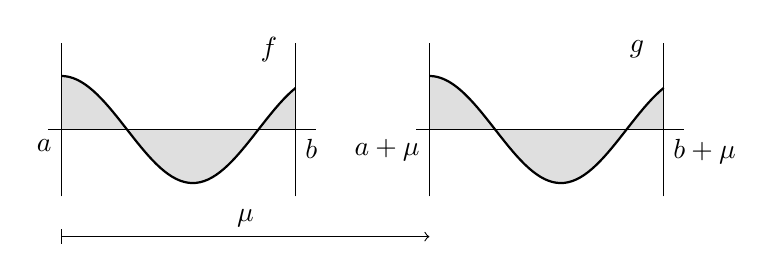
\begin{tikzpicture}[scale=0.85]
  \foreach \s/\n/\la/\lb in {0/f/a/b, 5.5/g/a+\mu/b+\mu}{
    \begin{scope}[xshift=\s cm]
      \fill[gray!25, domain=0:3.5, samples=60] plot (\x,{0.8*cos(deg(\x*1.6))}) -- (3.5,0) -- (0,0) -- cycle;
      \draw (-0.2,0) -- (3.8,0); \draw (0,-1) -- (0,1.3); \draw (3.5,-1) -- (3.5,1.3);
      \draw[thick, domain=0:3.5, samples=60] plot (\x,{0.8*cos(deg(\x*1.6))});
      \node at (3.1,1.2) {$\n$};
      \node[below left] at (0,0) {$\la$};
      \node[below right] at (3.5,0) {$\lb$};
    \end{scope}
  }
  \draw[|->] (0,-1.6) -- (5.5,-1.6) node[midway,above] {$\mu$};
\end{tikzpicture}
\end{center}

\begin{proposicion}
Si $f$ es integrable en $[a,b]$, entonces $g$ es integrable en $[a+\mu,b+\mu]$ y
\[
  \int_{a+\mu}^{b+\mu}g(y)\dd y\;\Bigl(=\int_{a+\mu}^{b+\mu}f(y-\mu)\dd y\Bigr)\overset{\text{Prop}}{=}\int_a^b f(x)\dd x.
\]
\end{proposicion}

\subsubsection*{2. Integración en espejo}

Sea $f\colon[a,b]\to\R$. Se define $g\colon[-b,-a]\to\R$ por
\[
  g(y):=f(-y)\qquad(\forall y\in[-b,-a]).
\]

\begin{center}
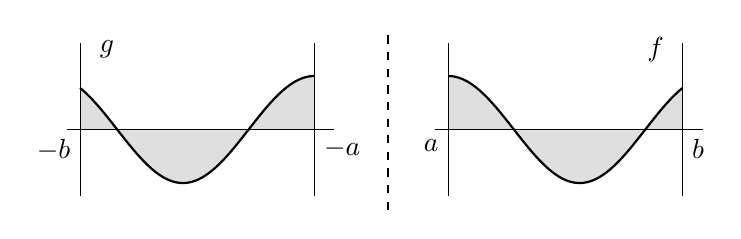
\begin{tikzpicture}[scale=0.85]
  \begin{scope}
    \fill[gray!25, domain=0:3.5, samples=60] plot (\x,{0.8*cos(deg((3.5-\x)*1.6))}) -- (3.5,0) -- (0,0) -- cycle;
    \draw (-0.2,0) -- (3.8,0); \draw (0,-1) -- (0,1.3); \draw (3.5,-1) -- (3.5,1.3);
    \draw[thick, domain=0:3.5, samples=60] plot (\x,{0.8*cos(deg((3.5-\x)*1.6))});
    \node at (0.4,1.2) {$g$};
    \node[below left] at (0,0) {$-b$};
    \node[below right] at (3.5,0) {$-a$};
  \end{scope}
  \draw[dashed] (4.6,-1.2) -- (4.6,1.5);
  \begin{scope}[xshift=5.5cm]
    \fill[gray!25, domain=0:3.5, samples=60] plot (\x,{0.8*cos(deg(\x*1.6))}) -- (3.5,0) -- (0,0) -- cycle;
    \draw (-0.2,0) -- (3.8,0); \draw (0,-1) -- (0,1.3); \draw (3.5,-1) -- (3.5,1.3);
    \draw[thick, domain=0:3.5, samples=60] plot (\x,{0.8*cos(deg(\x*1.6))});
    \node at (3.1,1.2) {$f$};
    \node[below left] at (0,0) {$a$};
    \node[below right] at (3.5,0) {$b$};
  \end{scope}
\end{tikzpicture}
\end{center}

\begin{proposicion}
Si $f$ es integrable en $[a,b]$, entonces $g$ es integrable en $[-b,-a]$, y
\[
  \int_{-b}^{-a}g(y)\dd y\;\Bigl(=\int_{-b}^{-a}f(-y)\dd y\Bigr)=\int_a^b f(x)\dd x
  \;\Longrightarrow\;
  \int_{-a}^{-b}g=-\int_a^b f.
\]
\end{proposicion}

\subsubsection*{3. Integración y dilatación}

Sea $f\colon[a,b]\to\R$. Dado $\lambda\ne0$, se considera la función
\[
  g\colon\begin{cases}
    [\lambda a,\lambda b]\to\R & \text{si } \lambda>0,\\
    [\lambda b,\lambda a]\to\R & \text{si } \lambda<0,
  \end{cases}
\]
definida por $g(y)=f(y/\lambda)$ $(\forall y\in[\lambda a,\lambda b])$.

\begin{center}
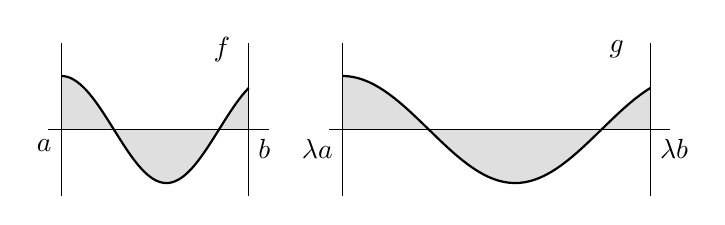
\begin{tikzpicture}[scale=0.85]
  \begin{scope}
    \fill[gray!25, domain=0:2.8, samples=60] plot (\x,{0.8*cos(deg(\x*2))}) -- (2.8,0) -- (0,0) -- cycle;
    \draw (-0.2,0) -- (3.1,0); \draw (0,-1) -- (0,1.3); \draw (2.8,-1) -- (2.8,1.3);
    \draw[thick, domain=0:2.8, samples=60] plot (\x,{0.8*cos(deg(\x*2))});
    \node at (2.4,1.2) {$f$};
    \node[below left] at (0,0) {$a$};
    \node[below right] at (2.8,0) {$b$};
  \end{scope}
  \begin{scope}[xshift=4.2cm]
    \fill[gray!25, domain=0:4.6, samples=60] plot (\x,{0.8*cos(deg(\x*2*2.8/4.6))}) -- (4.6,0) -- (0,0) -- cycle;
    \draw (-0.2,0) -- (4.9,0); \draw (0,-1) -- (0,1.3); \draw (4.6,-1) -- (4.6,1.3);
    \draw[thick, domain=0:4.6, samples=60] plot (\x,{0.8*cos(deg(\x*2*2.8/4.6))});
    \node at (4.1,1.2) {$g$};
    \node[below left] at (0,0) {$\lambda a$};
    \node[below right] at (4.6,0) {$\lambda b$};
  \end{scope}
\end{tikzpicture}
\end{center}

$f$ integrable en $[a,b]$ $\Rightarrow$ $g$ integrable en $[\lambda a,\lambda b]$ y
\[
  \int_{\lambda a}^{\lambda b}g(y)\dd y\;\Bigl(=\int_{\lambda a}^{\lambda b}f(y/\lambda)\dd y\Bigr)=\lambda\cdot\int_a^b f(x)\dd x.
\]

\subsection{Funciones escalonadas}

\begin{definicion}
Una función $f\colon[a,b]\to\R$ es \textbf{escalonada} si existe una partición
$P=\{a_0,a_1,\dots,a_n\}\subset[a,b]$ tal que $f$ es constante en cada subintervalo $(a_i,a_{i+1})$.
\end{definicion}

\begin{proposicion}
Toda función escalonada $f\colon[a,b]\to\R$ es integrable, y:
\begin{center}
$\displaystyle\int_a^b f=\sum_{i=0}^{n-1}(a_{i+1}-a_i)\,k_i$
\end{center}
donde $a_0,a_1,\dots,a_n$ son los puntos de la partición $P$ y $k_0,\dots,k_{n-1}$ son los valores tomados en los subintervalos $(a_0,a_1),\dots,(a_{n-1},a_n)$.
\end{proposicion}

\begin{ejercicio}
Sea $f\colon[a,b]\to\R$ acotada:
\begin{align*}
  I_*(f)&=\sup\Bigl\{\int_a^b s : s \text{ escalonada y } s\le f\Bigr\},\\
  I^*(f)&=\inf\Bigl\{\int_a^b t : t \text{ escalonada y } f\le t\Bigr\}.
\end{align*}
\end{ejercicio}

\begin{proposicion}
Sean $f,g\colon[a,b]\to\R$ tales que $f=g$, salvo en un número finito de puntos. Entonces $f$ es integrable si y sólo si $g$ lo es, y tienen misma integral.
\end{proposicion}

\begin{demo}
Sea $s:=g-f$. Tenemos que $s=0$, salvo en un número finito de puntos $a_0,a_1,\dots,a_n$
\[
  \Rightarrow s \text{ es escalonada, y } \int_a^b s=0.
\]
Luego: si $f$ es integrable $\Rightarrow f+s=g$ es integrable.
\end{demo}

\subsection{Integral de polinomios}

\begin{proposicion}
Dado $p\in\N$, la función $x\mapsto x^p$ es integrable en cualquier intervalo $[a,b]\subset\R$ y
\[
  \int_a^b x^p\dd x=\frac{b^{p+1}-a^{p+1}}{p+1}.
\]
\end{proposicion}

% ---------------------------------------------------------------------
\clase{16}{}{Integral de polinomios}
% ---------------------------------------------------------------------

\subsection{Integrales de las funciones polinomiales}

\begin{observacion}
Sea $f(x)=x^p$, con $p\in\N$.
\begin{itemize}
  \item Si $p$ es par: $f$ es monótona decreciente en $(-\infty,0]$ y creciente en $[0,+\infty)$.
  \item Si $p$ es impar: $f$ es monótona creciente en $\R$.
\end{itemize}
\end{observacion}

\begin{proposicion}
Dado $p\in\N$, la función $f(x)=x^p$ es integrable en cualquier intervalo $[a,b]$ (con $a<b$) y
\[
  \int_a^b x^p\dd x=\frac{b^{p+1}-a^{p+1}}{p+1}.
\]
\end{proposicion}

\begin{lema}
Para todos $x,y\in\R$ tales que $0\le x\le y$:
\[
  (y-x)\,x^p\le\frac{y^{p+1}-x^{p+1}}{p+1}\le(y-x)\,y^p.
\]
\end{lema}

\begin{demo}[Demostración del lema]
\begin{align*}
  (y-x)\sum_{i=0}^{p}x^iy^{p-i}
  &=(y-x)\bigl(y^p+xy^{p-1}+x^2y^{p-2}+\dots+x^{p-1}y+x^p\bigr)\\
  &=y^{p+1}+xy^p+x^2y^{p-1}+\dots+x^{p-1}y^2+x^py\\
  &\quad-xy^p-x^2y^{p-1}-x^3y^{p-2}-\dots-x^py-x^{p+1}\\
  &=y^{p+1}-x^{p+1}.
\end{align*}
Se observa
\begin{align*}
  \sum_{i=0}^{p}x^iy^{p-i}&\le\sum_{i=0}^{p}\overbrace{y^iy^{p-i}}^{y^p}=(p+1)\,y^p,\\
  \sum_{i=0}^{p}x^iy^{p-i}&\ge\sum_{i=0}^{p}\underbrace{x^ix^{p-i}}_{x^p}=(p+1)\,x^p.
\end{align*}
\[
  (p+1)\,x^p\le\sum_{i=0}^{p}x^iy^{p-i}\le(p+1)\,y^p
\]
\[
  x^p(p+1)(y-x)\le y^{p+1}-x^{p+1}\le(p+1)(y-x)\,y^p.
\]
\end{demo}

\begin{demo}[Demostración de la proposición]
Se distinguen 3 casos.

\textbf{Caso 1:} $0\le a<b$ \quad ($[a,b]\subset[0,+\infty)$).

Para toda partición $P=\{a_0,a_1,\dots,a_n\}\subset[a,b]$:
\begin{align*}
  S_*(f,P)&=\sum_{i=0}^{n-1}(a_{i+1}-a_i)\cdot a_i^p
  \le\sum_{i=0}^{n-1}\Bigl(\frac{a_{i+1}^{p+1}-a_i^{p+1}}{p+1}\Bigr)
  =\frac{a_n^{p+1}-a_0^{p+1}}{p+1}\\
  &=\frac{b^{p+1}-a^{p+1}}{p+1}.
\end{align*}
Luego: $I_*(f)\le\dfrac{b^{p+1}-a^{p+1}}{p+1}$.

Para toda partición $P=\{a_0,a_1,\dots,a_n\}\subset[a,b]$:
\[
  S^*(f,P)=\sum_{i=0}^{n-1}(a_{i+1}-a_i)\cdot a_{i+1}^p
  \ge\underbrace{\sum_{i=0}^{n-1}\frac{a_{i+1}^{p+1}-a_i^{p+1}}{p+1}}_{=\frac{b^{p+1}-a^{p+1}}{p+1}}.
\]
Luego: $I^*(f)\ge\dfrac{b^{p+1}-a^{p+1}}{p+1}$.

Conclusión:
\[
  \int_a^b x^p\dd x=I_*(f)=I^*(f)=\frac{b^{p+1}-a^{p+1}}{p+1}.
\]

\textbf{Caso 2:} $a<b\le0$ \quad ($[a,b]\subset(-\infty,0]$).
\[
  \int_a^b x^p\dd x=\int_{-b}^{-a}(-x)^p\dd x.
\]
\emph{Subcaso 2.1: $p$ es par.}
\begin{align*}
  \int_a^b x^p\dd x&=\int_{-b}^{-a}(-x)^p\dd x=\int_{-b}^{-a}x^p\dd x
  \overset{\text{caso 1}}{=}\frac{(-a)^{p+1}-(-b)^{p+1}}{p+1}\\
  &=\frac{-a^{p+1}+b^{p+1}}{p+1}=\frac{b^{p+1}-a^{p+1}}{p+1}.
\end{align*}
\emph{Subcaso 2.2: $p$ es impar.}
\begin{align*}
  \int_a^b x^p\dd x&=\int_{-b}^{-a}(-x)^p\dd x=-\int_{-b}^{-a}x^p\dd x
  =-\frac{(-a)^{p+1}-(-b)^{p+1}}{p+1}\\
  &=-\frac{a^{p+1}-b^{p+1}}{p+1}=\frac{b^{p+1}-a^{p+1}}{p+1}.
\end{align*}

\textbf{Caso 3:} $a<0<b$:
\[
  \int_a^b x^p\dd x=\int_a^0 x^p\dd x+\int_0^b x^p\dd x
  =\frac{0^{p+1}-a^{p+1}}{p+1}+\frac{b^{p+1}-0^{p+1}}{p+1}
  =\frac{b^{p+1}-a^{p+1}}{p+1}.
\]
\end{demo}

\begin{ejemplo}
Sea $f(x)=\frac{1}{3}x^3-x+1$. ¿$\displaystyle\int_{-1}^2 f$?
\begin{center}
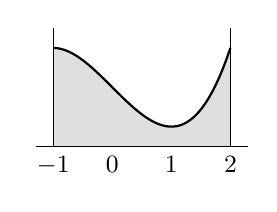
\begin{tikzpicture}[scale=0.75]
  \fill[gray!25, domain=-1:2, samples=50] (-1,0) -- plot (\x,{\x*\x*\x/3-\x+1}) -- (2,0) -- cycle;
  \draw (-1.3,0) -- (2.3,0);
  \draw (-1,0) -- (-1,2); \draw (2,0) -- (2,2);
  \draw[thick, domain=-1:2, samples=50] plot (\x,{\x*\x*\x/3-\x+1});
  \foreach \x in {-1,0,1,2} \node[below] at (\x,0) {\small$\x$};
\end{tikzpicture}
\end{center}
\begin{align*}
  \int_{-1}^2\Bigl(\tfrac13x^3-x+1\Bigr)\dd x
  &=\frac13\int_{-1}^2x^3\dd x-\int_{-1}^2x\dd x+\int_{-1}^2x^0\dd x\\
  &=\frac13\cdot\frac{2^4-(-1)^4}{4}-\frac{2^2-(-1)^2}{2}+\frac{2^1-(-1)^1}{1}=\frac{11}{4}.
\end{align*}
\end{ejemplo}

\[
  \int_a^b x^p\dd x=\frac{b^{p+1}-a^{p+1}}{p+1}=F(b)-F(a),
  \qquad\text{donde } F(x)=\frac{x^{p+1}}{p+1}.
\]
Se observa que $F'(x)=x^p$.

\begin{proposicion}
Si $f\colon\R\to\R$ es un polinomio, entonces
\[
  \int_a^b f\dd x=F(b)-F(a),
\]
donde $F$ es cualquier polinomio tal que $F'=f$.
\end{proposicion}

\begin{ejemplo}
$f(x)=\frac13x^3-x+1$, \qquad $F(x)=\dfrac{1}{12}x^4-\dfrac{x^2}{2}+x$ \qquad ($F'=f$).
\begin{center}
$\displaystyle\int_{-1}^2 f=F(2)-F(-1)=\frac{11}{4}$
\end{center}
\end{ejemplo}

% ---------------------------------------------------------------------
\clase{17}{}{Integral de 1/t y logaritmo}
% ---------------------------------------------------------------------

\subsection{Integral de $t\mapsto 1/t$}

Sea $f(t)=1/t$ para todo $t>0$ \quad ($f\colon\R^+\to\R$).

\textbf{Problema:} calcular $\displaystyle\int_a^b\frac{1}{t}\dd t$ para $0<a<b$.

\begin{observacion}
$f$ es monótona decreciente en $(0,+\infty)$: es localmente integrable.
\end{observacion}

\begin{proposicion}
Para todos $a,b,\lambda>0$ con $a<b$:
\[
  \int_{\lambda a}^{\lambda b}\frac{1}{t}\dd t=\int_a^b\frac{1}{t}\dd t.
\]
\end{proposicion}

\begin{demo}
Sea $f\colon[a,b]\to\R$ definida por $f(t)=\dfrac1t$. Se define $g\colon[\lambda a,\lambda b]\to\R$ por $g(t)=f(t/\lambda)=\dfrac{\lambda}{t}$.
\[
  \int_{\lambda a}^{\lambda b}g(t)\dd t=\int_{\lambda a}^{\lambda b}\frac{\lambda}{t}\dd t
  =\lambda\int_a^b f(t)\dd t=\lambda\int_a^b\frac1t\dd t,
\]
\[
  \int_{\lambda a}^{\lambda b}\frac{\lambda}{t}\dd t=\lambda\int_{\lambda a}^{\lambda b}\frac1t\dd t
  \quad\Rightarrow\quad
  \lambda\int_{\lambda a}^{\lambda b}\frac1t\dd t=\lambda\int_a^b\frac1t\dd t.
\]
\end{demo}

\begin{observacion}
$\displaystyle\int_a^b\frac1t\dd t$ no se puede expresar como un polinomio o una fracción racional en función de $a$ y de $b$.
\end{observacion}

\subsection{La función logaritmo}

\begin{definicion}
La \textbf{función logaritmo} es la función $\log\colon(0,+\infty)\to\R$ definida por
\[
  \log x:=\int_1^x\frac1t\dd t\qquad(\text{para todo } x>0).
\]
\end{definicion}

\begin{observacion}
Por definición, tenemos que
\[
  \log x=\begin{cases}
    \displaystyle\int_1^x\frac1t\dd t\ge0 & \text{si } x>1,\\[8pt]
    0 & \text{si } x=1,\\[4pt]
    -\displaystyle\int_x^1\frac1t\dd t\le0 & \text{si } x<1.
  \end{cases}
\]
\end{observacion}

\begin{proposicion}
La función logaritmo es estrictamente creciente en $(0,+\infty)$.
\end{proposicion}

\begin{demo}
Sean $x,y>0$ tales que $x<y$. Se observa que:
\[
  \log y-\log x=\int_1^y\frac1t\dd t-\int_1^x\frac1t\dd t=\int_x^y\frac1t\dd t\ge(y-x)\cdot\frac1y>0.
\]
Luego $\log x<\log y$.
\end{demo}

\subsubsection*{Propiedad fundamental del logaritmo}

$\forall\,x,y>0$:
\begin{enumerate}[label=(\arabic*)]
  \setcounter{enumi}{-1}
  \item $\log 1=0$
  \item $\log(xy)=\log x+\log y$
  \item $\log(x/y)=\log x-\log y$
  \item $\log(1/x)=-\log x$
\end{enumerate}

\begin{demo}[Demostración de (1)]
\[
  \log(xy)=\int_1^{xy}\frac1t\dd t=\int_1^x\frac1t\dd t+\int_x^{xy}\frac1t\dd t=\log(x)+\log(y).
\]
\end{demo}

\begin{demo}[Demostración de (2)]
$\log(x)=\log\bigl(y\cdot\frac{x}{y}\bigr)=\log y+\log\frac{x}{y}$. Luego: $\log\frac{x}{y}=\log x-\log y$.
\end{demo}

\begin{demo}[Demostración de (3)]
$\log\bigl(\frac1x\bigr)=\log(1)-\log(x)=-\log x$.
\end{demo}

\begin{proposicion}
Para todos $a,b>0$, tenemos que:
\[
  \int_a^b\frac1t\dd t=\log b-\log a=\log\frac{b}{a}.
\]
\end{proposicion}

\begin{demo}
\[
  \int_a^b\frac1t\dd t=\int_1^b\frac1t\dd t-\int_1^a\frac1t\dd t=\log b-\log a.
\]
\end{demo}

\begin{ejercicio}
Demostrar que $\forall x>0$:
\[
  1-\frac1x\le\log x\le x-1.
\]
\end{ejercicio}

\begin{solucion}
3 casos.
\begin{itemize}
  \item Caso $x=1$: $0\le0\le0$.
  \item Caso $x>1$: $\log x=\displaystyle\int_1^x\frac1t\dd t$. Para todo $t\in[1,x]$: $\dfrac1x\le\dfrac1t\le1$.
  \[
    \underbrace{(x-1)\cdot\frac1x}_{1-\frac1x}\le\int_1^x\frac1t\dd t\le\underbrace{(x-1)\cdot1}_{x-1}.
  \]
  \item Caso $x<1$: para todo $t\in[x,1]$ ($x\le t\le1$): $1\le\dfrac1t\le\dfrac1x$.
  \[
    (1-x)\cdot1\le\underbrace{\int_x^1\frac1t\dd t}_{-\log x}\le(1-x)\cdot\frac1x
  \]
  \[
    1-x\le-\log x\le\frac1x-1
    \;\Longleftrightarrow\;
    1-\frac1x\le\log x\le x-1.
  \]
\end{itemize}
\end{solucion}

\begin{ejercicio}
Demostrar que $\forall x>0$:
\begin{itemize}
  \item $\log\sqrt{x}=\frac12\log x$
  \item $\log(x^n)=n\cdot\log x$
  \item $\log\bigl(\sqrt[n]{x}\bigr)=\frac1n\log x$
\end{itemize}
\end{ejercicio}

\begin{solucion}\leavevmode
\begin{itemize}
  \item $x=\sqrt{x}\cdot\sqrt{x}$, \quad $\log x=\log\sqrt{x}+\log\sqrt{x}=2\log\sqrt{x}$ \quad $\Rightarrow\log\sqrt{x}=\frac12\log x$.
  \item $\displaystyle\log(x^n)=\log(\underbrace{x\cdot\ldots\cdot x}_{n\text{ veces}})
    =\underbrace{\log x+\dots+\log x}_{n\text{ veces}}=n\log x$
\end{itemize}
\end{solucion}

% =====================================================================
\end{document}
